\section{Design}
\label{sec:design}

This chapter presents the formal model and design method for Intent-Conditioned Value Projection, addressing the research questions and challenges set out in Chapter \ref{sec:aims}. We first state the threat model that the design has to contain, so that later safety claims can be read against a specific set of adversaries and failure modes. We then define ICVP as a decision model that treats stated user or governance intent as a projection over heterogeneous Internet of Value evidence spaces, and we state the two safety properties that link the model to the execution boundary. We then describe the agentic method that carries the model out, and the architecture that hosts it, including the account-level enforcement primitive (NFTAA) that realises trace-gated authorisation. The architecture follows from the formal model, not the other way round.

\subsection{Threat Model and Trust Assumptions}
\label{sec:threat-model}

The architecture combines components with very different trust properties. A safety claim is only as good as the adversary it is willing to name. Most on-chain losses have not come from cryptography or broken consensus. They come from a feed that quietly returned the wrong number, a model that read instructions out of retrieved content and followed them, a signing flow that swapped a transaction between approval and broadcast, or a person clicking through a confirmation they did not actually read. Those are the attackers the architecture has to survive. We do not try to defend against state-level adversaries or reorgs of the host chain.

The on-chain contracts are deterministic and inspectable, and we treat them as trusted once deployed. The validator and the \textit{RequiredEvidence} schemas are authored, content-addressed, and version-pinned, and we treat them as trusted under their documented key model. The language model in the proposer is opaque, replaceable, and not trusted to be correct. External evidence sources are untrusted in the worst case and lossy in the best case. Human approvers are trusted to authorise the actions they intend, but they are not assumed to be alert at three in the morning.

Table \ref{tab:threat-model} names the threats the design contains, marks the trust status of the affected component, and points to the mechanism that holds the line. Each row is referenced from at least one invariant in Section \ref{sec:proof-targets}, so the table is load-bearing rather than decorative.

\begin{table}[h]
\centering
\small
\begin{tabular}{|c|p{3.4cm}|p{3.0cm}|p{6.0cm}|}
\hline
\textbf{\#} & \textbf{Threat} & \textbf{Trust status of affected component} & \textbf{Containing mechanism} \\
\hline
T1 & Poisoned evidence (a source returns crafted content intended to flip the decision) & Evidence sources are untrusted & Schema requires multi-source corroboration and provenance per category. Validator rejects traces that rely on a single uncorroborated source for a decision-critical category. Hard constraints catch out-of-range values. \\
\hline
T2 & Stale evidence (data that was fresh when retrieved but is no longer fresh at authorisation time) & Evidence sources are untrusted, validator is trusted & Per-category freshness time-to-live values (TTLs) in the \textit{RequiredEvidence} schema, evaluated at authorisation time $t$, not at trace construction time. Section \ref{sec:proof-targets} states this as part of the Trace-Gated Authorisation property. \\
\hline
T3 & Prompt injection into the proposer (instructions embedded in retrieved evidence attempt to override the proposer's role) & Language model and retrieved text are untrusted & Proposer cannot emit a final decision. It can only emit a trace structured to the validator schema. Out-of-schema fields and free-text recommendations are dropped. The validator performs the gating check on structured fields, not on natural-language output. \\
\hline
T4 & Malicious or vague intent (a stated intent that does not correspond to the action being prepared, or that is too underspecified for a confident decision) & Intent comes from a trusted human but is not assumed correct & Intent is recorded as a structured input that drives the projection $P_i$. Underspecified intents fail schema requirements and force \textit{defer}. The transaction preparation step checks that the prepared transaction matches the trace, which in turn is bound to the recorded intent. \\
\hline
T5 & Manipulated oracles (price or risk feeds report manipulated values) & Oracles are untrusted & Schema specifies the oracle set per category, requires cross-feed agreement within a tolerance for decision-critical categories, and records each feed's provenance in the trace. NFTAA policy can additionally cap notional per action. \\
\hline
T6 & Incomplete traces (a trace that omits a required evidence category, or whose provenance is missing) & Proposer is untrusted, validator is trusted & Evidence-Completeness Safety in Section \ref{sec:proof-targets}. The validator refuses a confident \textit{proceed} unless \textit{RequiredEvidence}$(i, a) \subseteq E$ and provenance is recorded for every entry in $E$. \\
\hline
T7 & Transaction mismatch (a candidate transaction is submitted that does not correspond to the approved trace) & Transaction preparation is trusted-but-verified, signer environment is untrusted & The approval signature covers both the trace hash and the transaction hash. NFTAA verifies that the submitted transaction hashes to the value bound to the approval, and rejects otherwise. \\
\hline
T8 & Compromised agent process (the off-chain agent process is corrupted and emits arbitrary traces) & Off-chain runtime is untrusted at the boundary & Authority does not flow through the agent. The agent cannot authorise action. Only a human-approved, validator-signed trace bound to a policy-compliant transaction settles on-chain. A compromised agent can produce invalid traces, which the validator and NFTAA reject. \\
\hline
T9 & Policy bypass at NFTAA (an attempt to settle a value-relevant action without passing the on-chain policy) & NFTAA contract is trusted & The NFTAA contract is the sole settlement path for value-relevant actions of the account, and enforces the trace-gated authorisation checks of Section \ref{sec:proof-targets}. Direct asset transfers that bypass NFTAA are out of scope of the account's policy and out of scope of the safety claims. \\
\hline
T10 & Schema authorship attack (a weakened or replaced \textit{RequiredEvidence} schema lowers the bar for confident decisions) & Schemas are trusted authored artefacts & Schemas are versioned and content-addressed. The validator signs the trace jointly with the schema version and schema hash. NFTAA only accepts traces whose schema version is in a recognised set. Replacing the schema therefore breaks the signature rather than silently weakening the bar. \\
\hline
\end{tabular}
\caption[Threat model for the ICVP architecture]{Threat model for the ICVP architecture. Each row names a threat, the trust status of the affected component, and the mechanism that contains it. Safety properties in Section \ref{sec:proof-targets} reference the rows they depend on.}
\label{tab:threat-model}
\end{table}

Three assumptions sit outside the table because they bound the model rather than describe a threat. We assume at least one honest human approver per account, a validator key held under the operational model documented in Section \ref{sec:onchain-layer}, and a host chain whose consensus layer is not actively under attack at the moment we settle. If any of these break, the safety properties of Section \ref{sec:proof-targets} do not apply. We do not assume that the language model is correct, that any single evidence source is honest, that the off-chain runtime is uncompromised, or that the user's stated intent is the one they actually had in mind.

\subsection{Intent-Conditioned Value Projection}
\label{sec:icvp}

Value in the Internet of Value is heterogeneous and context-dependent. Lohmer et al. \cite{Lohmer2024} reach a comparable conclusion through expert interviews, arguing that value in this setting cannot be reduced to market price and instead spans economic worth, utility or access rights, and ethical and sustainability contributions. The same observation appears whenever we look across asset classes. A Pudgy Penguin held for community access is not valued in the same terms as the same Pudgy Penguin held for short-term resale. stETH evaluated as productive collateral is not valued in the same terms as stETH evaluated for liquidity exit during a peg dislocation. A Polkadot OpenGov proposal evaluated under public-resource stewardship is not valued in the same terms as a private acquisition. In each case the asset is the same. The intent is different, and so are the evidence that matters and the way Availability, Durability, and Utility are interpreted.

We therefore propose Intent-Conditioned Value Projection (ICVP) as the decision model. ICVP treats stated user or governance intent as a projection over heterogeneous Internet of Value evidence spaces. The projection determines what evidence is relevant, after which Availability, Durability, and Utility are instantiated for the asset class and the action context. ICVP does not require predefined asset-specific value formulas for previously unseen asset classes. It requires an intent-specific projection over available evidence and an intent-specific instantiation of the three valuation dimensions on top of that projection.

Let $a$ be an asset, proposal, or value-relevant object in the Internet of Value. Examples include a non-fungible token, a liquid staking token such as stETH, a treasury proposal, a tokenised claim, an access right, a redemption right, or a public-good funding request. Let $E$ be the available evidence set for $a$. Evidence in this setting can include price and liquidity, supply and rarity, metadata storage and contract mutability, governance and access rights, redemption rights, yield source, protocol risk, counterparty risk, compliance status, public-good contribution, team and delivery history, audit reports, on-chain footprint, and provenance information. We write $F(a, E)$ for the full feature space derived from $a$ and $E$.

Let $i$ be a stated intent. Intent in ICVP is not an attempt to model human psychology. It is a declared computational input that constrains what evidence is relevant and how the valuation dimensions are instantiated. Examples include long-term holding, speculative trading, collateralisation, functional or community access, liquidity exit, protocol-risk evaluation, treasury stewardship, and so on. Let $P_i$ be an intent-specific projection that selects and transforms the parts of $F(a, E)$ that are relevant under $i$:
\begin{equation}
F_i(a, E) = P_i(F(a, E)).
\end{equation}
Let $\Phi_i$ instantiate the three valuation dimensions from the projected evidence:
\begin{equation}
\Phi_i(F_i(a, E)) = (A_i, D_i, U_i),
\end{equation}
where $A_i$, $D_i$, and $U_i$ are the intent-instantiated Availability, Durability, and Utility for $a$ under $i$. The decision signal is then computed by an intent-specific aggregation:
\begin{equation}
V_i = g_i(A_i, D_i, U_i).
\end{equation}
A common operational choice for $g_i$ is the convex combination
\begin{equation}
g_i(A_i, D_i, U_i) = w_A(i) \cdot A_i + w_D(i) \cdot D_i + w_U(i) \cdot U_i,
\label{eq:adu-aggregation}
\end{equation}
with weights $w_A(i), w_D(i), w_U(i) \in [0, 1]$ and $w_A(i) + w_D(i) + w_U(i) = 1$, and with each $A_i, D_i, U_i \in [0, 10]$ for interpretability. We use this aggregation in the implementation, but we treat it as an aggregator over already intent-instantiated dimensions, not as the value model itself. Aggregation alone, without the projection $P_i$ and the instantiation $\Phi_i$, reduces to a fixed-weight scoring heuristic of the kind we evaluate against as a baseline in Chapter \ref{sec:evaluation}.

The full output of ICVP for asset $a$ under intent $i$ given evidence $E$ is
\begin{equation}
\textsc{ICVP}(a, i, E) = (F_i, A_i, D_i, U_i, V_i, d, \tau),
\end{equation}
where $d \in \{\textit{proceed}, \textit{defer}, \textit{decline}\}$ is the decision and $\tau$ is the auditable valuation trace. The labels are interpreted operationally. \textit{Proceed} means the projected evidence supports the action under the stated intent. \textit{Defer} means the projected evidence is missing, stale, or conflicting, or confidence is below threshold. \textit{Decline} means the evidence does not justify the action or a hard constraint blocks it. The trace $\tau$ records the stated intent, the selected evidence with its provenance, the deprioritised evidence where relevant, the intent-specific interpretation of $A_i$, $D_i$, and $U_i$, the scores or qualitative judgements, the confidence, the hard constraints, the decision, and a link to any prepared transaction. The trace is a structured artefact meant to be inspected rather than read as narrative. A deterministic validator checks it for required evidence, provenance, and policy compatibility before any human approval step.

In our setting Availability, Durability, and Utility remain the practical valuation taxonomy across asset classes, but their content depends on intent. Availability for a Pudgy Penguin under speculative trading involves floor price, listing depth, recent sales, and market liquidity. Availability for the same Pudgy Penguin under community access involves access rights, membership scarcity, and the existence of comparable communities reachable through other tokens. Availability for stETH under collateralisation involves DeFi liquidation depth and accepted collateral lists rather than NFT-style rarity. Availability for a treasury proposal under public-resource stewardship involves whether comparable contributions already exist, whether alternative teams can deliver the work, and the opportunity cost of the requested treasury allocation. Durability for an NFT held long-term centres on metadata storage guarantees, smart-contract immutability, and ecosystem resilience. Durability for stETH held long-term centres on validator decentralisation, slashing exposure, and protocol governance stability. Durability for a treasury proposal centres on maintainability of the deliverables, sustainability of the funded team, and stability of dependencies. Utility for an NFT under functional use centres on access, brand, and in-product utility. Utility for stETH under productive use centres on yield source, composability with lending and trading venues, and reliability of the redemption path. Utility for a treasury proposal under stewardship centres on ecosystem benefit, public-good impact, and strategic alignment. The valuation taxonomy is shared across these cases, but the projection and the instantiation are not.

The agent in this architecture is not the source of value. It is an evidence interpreter and trace proposer. It maps asset features and stated intent into an auditable valuation trace, and a deterministic validator together with human approval and account-level policy decide whether the trace can authorise an on-chain action. Section \ref{sec:proof-targets} states the safety properties that link the formal model to the execution boundary. The Internet of Value makes assets transferable, and ICVP is what makes their value interpretable under a stated intent.

\subsubsection{Formal proof targets}
\label{sec:proof-targets}

The formal scope of this thesis is deliberately narrower than a theory of value. We do not attempt to prove that an underlying language model is correct, that a \textit{proceed} decision is objectively true, or that expert evaluators are absolute ground truth. We instead target two safety properties that connect the ICVP decision model to the execution boundary enforced by NFTAA in Section \ref{sec:onchain-layer}.

The first property is \emph{Evidence-Completeness Safety}. Let $\theta$ be the confidence threshold for confident decisions and let $\textit{RequiredEvidence}(i, a)$ denote the intent-specific evidence required for asset $a$ under intent $i$. Then
\begin{equation}
\begin{aligned}
&\textsc{Decision}(a, i, E) = \textit{proceed}
  \;\wedge\; \textsc{Confidence}(a, i, E) \geq \theta \\
&\qquad\Longrightarrow\;
  \textit{RequiredEvidence}(i, a) \subseteq E
  \;\wedge\; \textsc{Provenance}(E).
\end{aligned}
\end{equation}
The contrapositive is the operationally useful form. If the required intent-specific evidence is missing, the system must not return a confident \textit{proceed}. It must lower confidence, defer, or decline. Under this property the valuation trace functions as a checked artefact rather than as a narrative. This property contains threats T1, T3, and T6 of Table \ref{tab:threat-model}, in the sense that poisoned evidence, prompt-injection attempts that bypass the trace structure, and incomplete traces cannot lead to a confident \textit{proceed}.

The second property is \emph{Trace-Gated Authorisation}. A value-relevant transaction $\textit{tx}$ submitted at authorisation time $t$ can be authorised only if there exists a trace $\tau$ such that
\begin{equation}
\begin{aligned}
&\textsc{Authorise}(\textit{tx}, t)
  \;\Longrightarrow\; \exists \tau: \\
&\qquad \textsc{ValidTrace}(\tau)
  \,\wedge\, \textsc{CompleteEvidence}(\tau, i) \\
&\qquad \wedge\, \textsc{Decision}(\tau) = \textit{proceed}
  \,\wedge\, \textsc{FreshEvidence}(\tau, t) \\
&\qquad \wedge\, \textsc{NotExpired}(\tau, t)
  \,\wedge\, \textsc{TxMatches}(\textit{tx}, \tau) \\
&\qquad \wedge\, \textsc{PolicyAllows}(\textit{tx}, \tau).
\end{aligned}
\end{equation}
The freshness predicates are evaluated at the authorisation moment, not at the trace-construction moment. $\textsc{FreshEvidence}(\tau, t)$ holds iff, for every evidence category $c$ used by $\tau$, the recorded acquisition timestamp $\textit{acq}_c$ satisfies $t - \textit{acq}_c \leq \textit{TTL}_c$, where $\textit{TTL}_c$ is the time-to-live for category $c$ recorded in the \textit{RequiredEvidence} schema used by $\tau$. Per-category TTLs are stated in orders of magnitude that match the underlying signal: market and liquidity data in minutes, oracle and peg readings in minutes, protocol-risk signals such as audit status or validator-set composition in days, and team-history or governance-record signals in months. $\textsc{NotExpired}(\tau, t)$ holds iff the trace itself has not crossed its own expiry, which is the minimum of the per-category TTL horizons and the policy expiry.

This couples the formal value model to policy-constrained execution. The proof can be carried out over an abstract state machine with active policies, schema versions, evidence requirements with per-category TTLs, valuation traces, approvals, nonces, the current time, and authorised and executed transactions. The key transition is the authorisation transition, which fires at time $t$ and requires a valid trace with complete evidence, a \textit{proceed} decision, a trace-matching transaction, a permitting policy, evidence still fresh at $t$, a trace not yet expired at $t$, a fresh nonce, and a non-revoked policy. The trace-built-then-stale case is handled explicitly. A trace $\tau$ that satisfied $\textsc{FreshEvidence}$ when constructed at time $t_0$ but no longer satisfies $\textsc{FreshEvidence}$ at $t > t_0$ falls out of the authorisation transition, because the predicate is evaluated against $t$. The trace can be rebuilt, but it cannot be replayed past its evidence horizon. Section \ref{sec:trace-commitment} specifies the commitment scheme that realises the freshness predicate on-chain, and Section \ref{sec:onchain-layer} returns to this property and specifies the NFTAA-level checks that realise it. This property contains threats T2, T5, T6, T7, T8, T9, and T10 of Table \ref{tab:threat-model}, in the sense that stale evidence, manipulated oracles, incomplete traces, transaction mismatch, a compromised agent process, attempts to bypass NFTAA, and schema substitution cannot lead to authorisation.

We do not prove that an authorised transaction is the right transaction. We prove that no transaction can be authorised without a valid trace, fresh evidence at authorisation time, a recognised schema version, and a permitting policy. The narrower claim is the one we believe the architecture can defensibly support, even when the agent acts only as an evidence interpreter and recommendation generator.

\subsubsection{RequiredEvidence schemas as authored artefacts}
\label{sec:required-evidence-schemas}

The predicate $\textit{RequiredEvidence}(i, a)$ that appears in both safety properties is not an output of the language model. It is an authored, versioned artefact that is part of the contribution of this thesis. We make this status explicit because it is what allows the validator to be deterministic, the proof targets to be stated as predicates over states rather than over generations, and the on-chain check to recognise a schema version rather than to trust whatever the off-chain runtime claims to have used.

A \textit{RequiredEvidence} schema is a structured document keyed by intent and asset class. Each schema declares a schema version, an asset-class identifier, an intent identifier, a list of required evidence categories, a list of optional categories that strengthen confidence when present, a freshness time-to-live $\textit{TTL}_c$ per category, provenance requirements per category, hard constraints expressed as predicates over recorded values, and a citation list naming the sources from which the requirements are drawn. The version field is mandatory. The validator signs the schema version and the schema hash jointly with the trace hash as described in Section \ref{sec:trace-commitment}, and the on-chain check refuses traces whose schema version is not in the contract's recognised set. The evaluation harness records the schema version used by each task as a configuration field, so that any reported result can be reproduced against the same schema bytes.

We author one schema per regime in the evaluation, with sources cited inline so that every requirement is traceable. The NFT or access regime draws its categories from the hedonic-pricing and rarity literature on NFT valuation \cite{Lohmer2024, Ante2021, Dowling2022, Nadini2021, Kong2021}, together with metadata and provenance evidence from the contract and on-chain history. The productive-asset regime draws its categories from liquid-staking and DeFi risk analyses \cite{frangella2022aave, gambacorta2024defi} and from the public Lido risk disclosure on validator-set composition, slashing exposure, and withdrawal queue behaviour \cite{LidoRisk}. The treasury-governance regime draws its categories from the Web3 Foundation OpenGov treasury voting guidelines and from the academic and practitioner literature on treasury proposal evaluation \cite{W3FOpenGovVotingGuidelines, Rodrigues2022, Valastin2024proto}. The full schemas, with all fields and source citations, are listed in Appendix \ref{app:required-evidence-schemas}.

Because the schemas are part of the contribution, they are also part of the evaluation. We run the main evaluation against the authored schemas at their tagged versions. We also run an additional comparison condition against a deliberately weakened variant of each schema, in which provenance requirements are relaxed, two of the required categories are demoted to optional, and the freshness TTLs are loosened by an order of magnitude. The weakened variant is tagged as its own schema version so that the on-chain check would refuse it if it were not in the recognised set. The purpose of the weakened condition is to test whether ICVP still beats the reduced valuation baselines when the schema is unfavourable to it. If the gap collapses, the contribution depends on schema authorship rather than on the projection $P_i$ and the instantiation $\Phi_i$. If the gap survives, the contribution holds at the level we claim.

\subsubsection{Trace commitment and on-chain verification}
\label{sec:trace-commitment}

The two safety properties are stated above as predicates over abstract states. Realising them at the execution boundary requires a commitment scheme that the on-chain layer can check without trusting the off-chain runtime. We describe that scheme here. Section \ref{sec:onchain-layer} returns to the same checks from the NFTAA side.

\paragraph{Off-chain trace storage.}
The valuation trace $\tau$ is stored off-chain in a content-addressed store, addressed by $\textit{cid}(\tau) = \textsc{Hash}(\tau)$. IPFS is the reference choice in the prototype, but any content-addressed store with the same integrity property is admissible. Storing $\tau$ off-chain keeps the on-chain footprint small, and storing it content-addressed makes the on-chain hash a binding commitment to the bytes that the validator and the human approver saw.

\paragraph{Schema commitment and validator signature.}
The validator signs the trace jointly with its schema version and schema hash, not separately. Let $\textit{ver}(\tau)$ be the schema version that $\tau$ was validated against and let $\textit{sh}(\tau) = \textsc{Hash}(\textit{schema}_{\textit{ver}(\tau)})$ be the content hash of that schema. The validator emits
\[
\sigma_V \;=\; \textsc{Sign}_{\textit{sk}_V}\bigl(\textsc{Hash}(\tau)\,\|\,\textit{ver}(\tau)\,\|\,\textit{sh}(\tau)\bigr).
\]
Joint signing has the property that an attempt to retroactively weaken the schema breaks $\sigma_V$, because $\textit{sh}(\tau)$ would no longer match the signed value. This contains threat T10 of Table \ref{tab:threat-model}. The validator key $\textit{sk}_V$ is documented separately. A single validator key is acceptable for the prototype and is the configuration we use. The associated trust assumption is that $\textit{sk}_V$ is held in a way consistent with the trust assumptions of Section \ref{sec:threat-model}. A multi-validator or threshold configuration is a straightforward extension and does not change the safety statements.

\paragraph{Approval signature.}
The human approver signs the trace hash and the transaction hash jointly, not in sequence. Let $\textit{tx}$ be the candidate transaction. The approver emits
\[
\sigma_H \;=\; \textsc{Sign}_{\textit{sk}_H}\bigl(\textsc{Hash}(\tau)\,\|\,\textsc{Hash}(\textit{tx})\bigr).
\]
Joint signing has the property that an attempt to swap the transaction after approval breaks $\sigma_H$, because $\textsc{Hash}(\textit{tx})$ would no longer match the signed value. This contains threat T7 of Table \ref{tab:threat-model}.

\paragraph{NFTAA on-chain check.}
At authorisation time $t$, the NFTAA contract performs the following checks in order. Each check corresponds to a conjunct of the Trace-Gated Authorisation property.
\begin{enumerate}
    \item \textbf{Hash match.} The submitted $\textit{tx}$ references a trace commitment $\textit{cid}(\tau)$ and the contract checks $\textit{cid}(\tau) = \textsc{Hash}(\tau)$ against the value bound to the approval. (Realises $\textsc{ValidTrace}$ and $\textsc{TxMatches}$.)
    \item \textbf{Schema version recognised.} The schema version $\textit{ver}(\tau)$ is in the contract's accepted-version set and the recorded $\textit{sh}(\tau)$ matches the version's registered hash. (Contains T10.)
    \item \textbf{Validator signature.} $\textsc{Verify}_{\textit{pk}_V}(\sigma_V, \textsc{Hash}(\tau)\,\|\,\textit{ver}(\tau)\,\|\,\textit{sh}(\tau))$ holds. (Realises $\textsc{ValidTrace}$ jointly with the previous step.)
    \item \textbf{Approval signature.} $\textsc{Verify}_{\textit{pk}_H}(\sigma_H, \textsc{Hash}(\tau)\,\|\,\textsc{Hash}(\textit{tx}))$ holds, for an approver key recognised by the account's policy. (Contains T7.)
    \item \textbf{Policy match.} The actor, asset, target contract, function selector, amount, and chain identifier of $\textit{tx}$ fall inside the active policy. (Realises $\textsc{PolicyAllows}$, contains T9.)
    \item \textbf{Fresh nonce.} The trace-bound nonce has not been used by this account. (Replay protection.)
    \item \textbf{Not expired.} $t$ is not past the trace expiry $\textit{exp}(\tau)$ or the policy expiry. (Realises $\textsc{NotExpired}$, contains T2.)
    \item \textbf{Not revoked.} The policy has not been revoked at time $t$. (Closes the time-of-check to time-of-use gap on the policy side.)
\end{enumerate}
Settlement happens only when all eight checks hold. If any check fails the call reverts and no state change is committed. The freshness predicate $\textsc{FreshEvidence}(\tau, t)$ is enforced as part of step seven on the NFTAA side, because $\textit{exp}(\tau)$ is computed off-chain as the minimum of the per-category TTL horizons and is recorded in $\tau$ before validator signing. An attempt to relax $\textit{exp}(\tau)$ after signing breaks $\sigma_V$. The eight checks together realise the Trace-Gated Authorisation property at the execution boundary. The detailed call sequence for the prototype, including the signing pipeline and the NFTAA call sites, is presented in the implementation chapter alongside the contract code.

\subsection{Design Decisions and Rejected Alternatives}
\label{sec:design-decisions}

The architecture we present is one of several defensible designs. Before turning to the methodology, we make the alternatives explicit and explain why we rejected them, so that the reasoning that shaped ICVP and its enforcement boundary is visible to the reader rather than implicit in the result. We focus on the three decisions that most directly determine the formal shape of the contribution. The remaining design choices, including the role of \textit{defer}, the placement of human approval, the function of NFTAA, the evaluation protocol, and the proof scope, are stated where they have the strongest bearing on the chapters that follow.

\paragraph{Decision 1: Intent as projection over evidence, not weights over fixed dimensions.}
The simpler alternative we considered first treats Availability, Durability, and Utility as fixed variables and lets intent only re-weight them, as in
\[
V_i(a) = w_A(i)\, A(a) + w_D(i)\, D(a) + w_U(i)\, U(a).
\]
This formulation is attractive because it keeps the valuation function closed-form and the contribution of intent reduces to a single vector of weights. We rejected it for two reasons that are structural rather than aesthetic. First, the formulation presupposes that the same empirical variables are the right ones for every intent and every asset class. For heterogeneous Internet of Value objects, this is not the case. A Pudgy Penguin acquired for community access, an stETH position held for productive yield, and a Polkadot OpenGov treasury proposal evaluated under public-resource stewardship do not surface comparable evidence at all. The metadata permanence of a collectible, the peg depth and withdrawal queue of a liquid staking derivative, and the milestone schedule of a treasury proposal are not three measurements of one quantity. Reweighting cannot reconcile evidence that is categorically different. Second, the same object changes the evidence that matters under different intents. For an NFT held for long-term community access, metadata permanence and contract upgradeability dominate. For the same NFT used as DeFi collateral, oracle robustness, market depth at the relevant tick, and liquidation behaviour dominate instead. A fixed-dimension model cannot represent the fact that intent reshapes what counts as evidence, not only how much it counts. We therefore treat intent as an explicit projection $P_i$ over the evidence space $F(a, E)$, and only after projection do we instantiate $A_i, D_i, U_i$ on the projected evidence. The valuation $V_i = g_i(A_i, D_i, U_i)$ is the last step rather than the model. Our contribution is consequently a formal account of how stated intent changes evidence relevance and the empirical meaning of the valuation dimensions, not a parameterisation of weights on top of pre-fixed dimensions.

\paragraph{Decision 2: A/D/U as an intent-instantiated taxonomy, not a universal ontology.}
A second alternative we considered is to present Availability, Durability, and Utility as a universal ontology with one fixed empirical meaning per dimension across all asset classes. The appeal of this position is methodological economy. A universal ontology offers a single coordinate system in which any value object can be located, and it suggests that valuation reduces to measuring three well-defined quantities. We rejected this position because the tidiness is superficial. Under a universal ontology, Availability would have to mean the same operational quantity for an illiquid collectible, a deeply liquid staking derivative, and a treasury proposal whose Availability is not market liquidity at all but the scarcity or under-supply of the public-good contribution being requested. The shared label would hide incompatible measurements behind a single name, and any cross-asset comparison conducted on top of that label would be unsound. We retain Availability, Durability, and Utility because they are a useful taxonomy for thinking about value across the Internet of Value, but we make their empirical content depend on intent. For an NFT held for community access, Availability is rarity and access scarcity, Durability is metadata permanence and contract upgradeability, and Utility is membership benefit and cultural relevance. For stETH held for productive yield, Availability is liquidity and peg depth, Durability is validator-set health and protocol governance risk, and Utility is the realised yield net of fees and slashing exposure. For a Polkadot OpenGov treasury proposal, Availability is the scarcity of the proposed contribution and the opportunity cost of the requested allocation, Durability is the sustainability of the funded deliverables, and Utility is ecosystem benefit and strategic alignment. The taxonomy stays the same across the three cases, but its content is reset by the stated intent. This lets us preserve comparability of structure across cases without committing to the false claim that one coordinate system fits every value object.

\paragraph{Decision 3: Evidence-grounded valuation with a deterministic validator, not direct agent recommendation.}
The third alternative we considered is the operationally simplest. We could let a language model read the asset, the intent, and the retrieved context, and emit \textit{proceed}, \textit{defer}, or \textit{decline} directly. We rejected this design because it confuses the source of evidence with the source of authority. If the model is the recommender, the dissertation must defend the recommendation, and the recommendation depends on opaque generation behaviour that we cannot characterise formally. The defence would have to take the form of a claim about model behaviour in general, which neither the literature nor our own evaluation can support at the level of rigour a value-relevant on-chain action requires. We instead split the role of the agent into two functions that can be inspected separately. The agent is an evidence interpreter and trace proposer. It retrieves evidence under the projection $P_i$, maps evidence to features that are relevant under the stated intent, proposes intent-conditioned instantiations of $A_i, D_i, U_i$, and assembles a valuation trace $\tau$ that records the evidence used, its provenance, the projection applied, the dimension instantiations, the resulting $V_i$, the decision, and the confidence. A separate deterministic validator then checks the trace for evidence completeness against $\textit{RequiredEvidence}(i, a)$, provenance, schema validity, hard constraints, and internal consistency. The trace is the unit that downstream stages reason about, and the validator is what gates whether the trace can support a confident decision. This separation lets us state the safety properties of Section \ref{sec:proof-targets} cleanly. We do not need to argue that the language model is correct. We only need the property that no confident \textit{proceed} can be returned, and no transaction can be authorised, without required evidence, a valid trace, human approval, and a permitting policy. The narrower claim is what we believe the architecture can defensibly support, and the validator is the artefact that makes the claim checkable.

\subsection{Methodology proposal}

The methodology puts ICVP into practice. It transforms a stated intent and an asset into an auditable valuation trace and, when applicable, into a policy-constrained transaction prepared for human approval and account-level enforcement. Each phase maps to a distinct architectural layer, so the pipeline from intent to settlement is explicit rather than implicit. The methodology follows the formal model in Section \ref{sec:icvp}, which guarantees that the projection $P_i$ and the instantiation $\Phi_i$ are visible steps in the pipeline rather than hidden assumptions inside a single prompt.

We propose the following setup for asset valorisation in agentic systems within the Internet of Value:

\begin{enumerate}
    \item \textbf{Evidence acquisition.} Given the asset $a$ and the stated intent $i$, the agent retrieves evidence $E$ from external data sources and records provenance for each item. The retrieval is intent-aware, so the evidence pulled for community access differs from the evidence pulled for speculative trading even when the asset is the same.
    \item \textbf{Intent-specific projection and instantiation.} The agent applies the intent-specific projection $P_i$ to the retrieved evidence and instantiates $A_i$, $D_i$, and $U_i$ for the asset class and the action context. This step makes explicit what counts as Availability, Durability, and Utility under $i$.
    \item \textbf{Trace construction and decision.} The agent assembles the valuation trace $\tau$, computes the decision signal $V_i$ and the decision $d \in \{\textit{proceed}, \textit{defer}, \textit{decline}\}$, and attaches confidence and hard constraints. A deterministic validator checks the trace for required evidence, provenance, and policy compatibility.
    \item \textbf{Approval and policy-constrained execution.} Once a human approves the action, the execution component prepares an on-chain transaction linked to $\tau$ and submits it to the NFTAA-controlled account. The account-level policy enforces the trace-gated authorisation property of Section \ref{sec:proof-targets} before any state change is settled on-chain.
\end{enumerate}


In the following subsection, we will describe the technical and operational requirements for a functional architecture for agentic systems in the context of the Internet of Value and NFTs. Requirements are organized systematically, into four categories: data acquisition, agent capabilities, execution guarantees, and security properties.

\subsection{System Requirements}


To instantiate the projected dimensions $A_i$, $D_i$, and $U_i$ for an asset $a$ under a stated intent $i$, the system must acquire heterogeneous data from multiple sources. The data acquisition layer does not decide what is relevant. The intent-specific projection $P_i$ does. Data acquisition only needs to make a sufficient evidence space available so that $P_i$ can select from it. Therefore, we define the following data acquisition requirements:

\begin{itemize}
    \item The system should retrieve data from at least one data source, namely: Blockchain explorers, Decentralized storage networks, Marketplace APIs, Rarity analytics, and Oracle services.
    \item Data from heterogeneous sources must be normalized into a canonical schema that enables cross-asset comparison. For example, metadata from OpenSea, LooksRare, and native IPFS retrieval must be transformed into a standard JSON structure with standardized field names.
    \item Each data point should be accompanied by provenance information: the source URL, retrieval timestamp, and content hash. This ensures verifiability and auditability of the acquired information.
\end{itemize}

The system needs the following capabilities to analyse assets and prepare decisions under a stated intent.

\begin{itemize}
    \item Accept user or governance intent in natural language and record it as a structured input that drives the projection $P_i$ and the instantiation $\Phi_i$ defined in Section \ref{sec:icvp}.
    \item Given an asset identifier and a stated intent, retrieve the evidence permitted by $P_i$, instantiate Availability, Durability, and Utility for the asset class and the action context, and emit a structured rationale for each dimension. Weighted aggregation, when used, runs only after projection and instantiation, and is one operational choice, not the value model.
    \item Produce a structured valuation trace, including a decision in $\{\textit{proceed}, \textit{defer}, \textit{decline}\}$, that a deterministic validator can check for required evidence, provenance, and policy compatibility.
    \item Do not authorise execution on its own. The transaction preparation component constructs, simulates, and packages a candidate transaction linked to the trace, presents it for human approval, and submits it to the on-chain layer only after approval has been recorded. Account-level policy checks (spending limits, allowed protocols, evidence and trace conditions) stay enforced on-chain.
\end{itemize}


\subsection{Architecture}

The architecture connects human intent with blockchain settlement through three operational layers (local, agentic, and on-chain), supported by an external data layer that supplies market, metadata, governance, and oracle inputs. The pipeline runs in one direction: Intent $\rightarrow$ ICVP $\rightarrow$ Valuation Trace $\rightarrow$ Human Approval $\rightarrow$ NFTAA Policy Check $\rightarrow$ On-chain Execution. The local layer is where a participant states intent in natural language, which is verified and turned into a structured input. The agentic layer retrieves the projected evidence, instantiates Availability, Durability, and Utility under the stated intent, assembles a valuation trace, and runs deterministic validation. After a human approves a specific candidate transaction linked to a valid trace, the transaction preparation component submits it to the on-chain layer. The on-chain layer, anchored by NFTAA, runs the policy check and settles the action only when the trace, the human approval, and the policy all permit it. The data layer is an external dependency, not a fourth execution layer. It does not reason about value and does not move funds. It supplies the inputs the agentic layer reads.

\begin{figure}[!h]
    \centering
    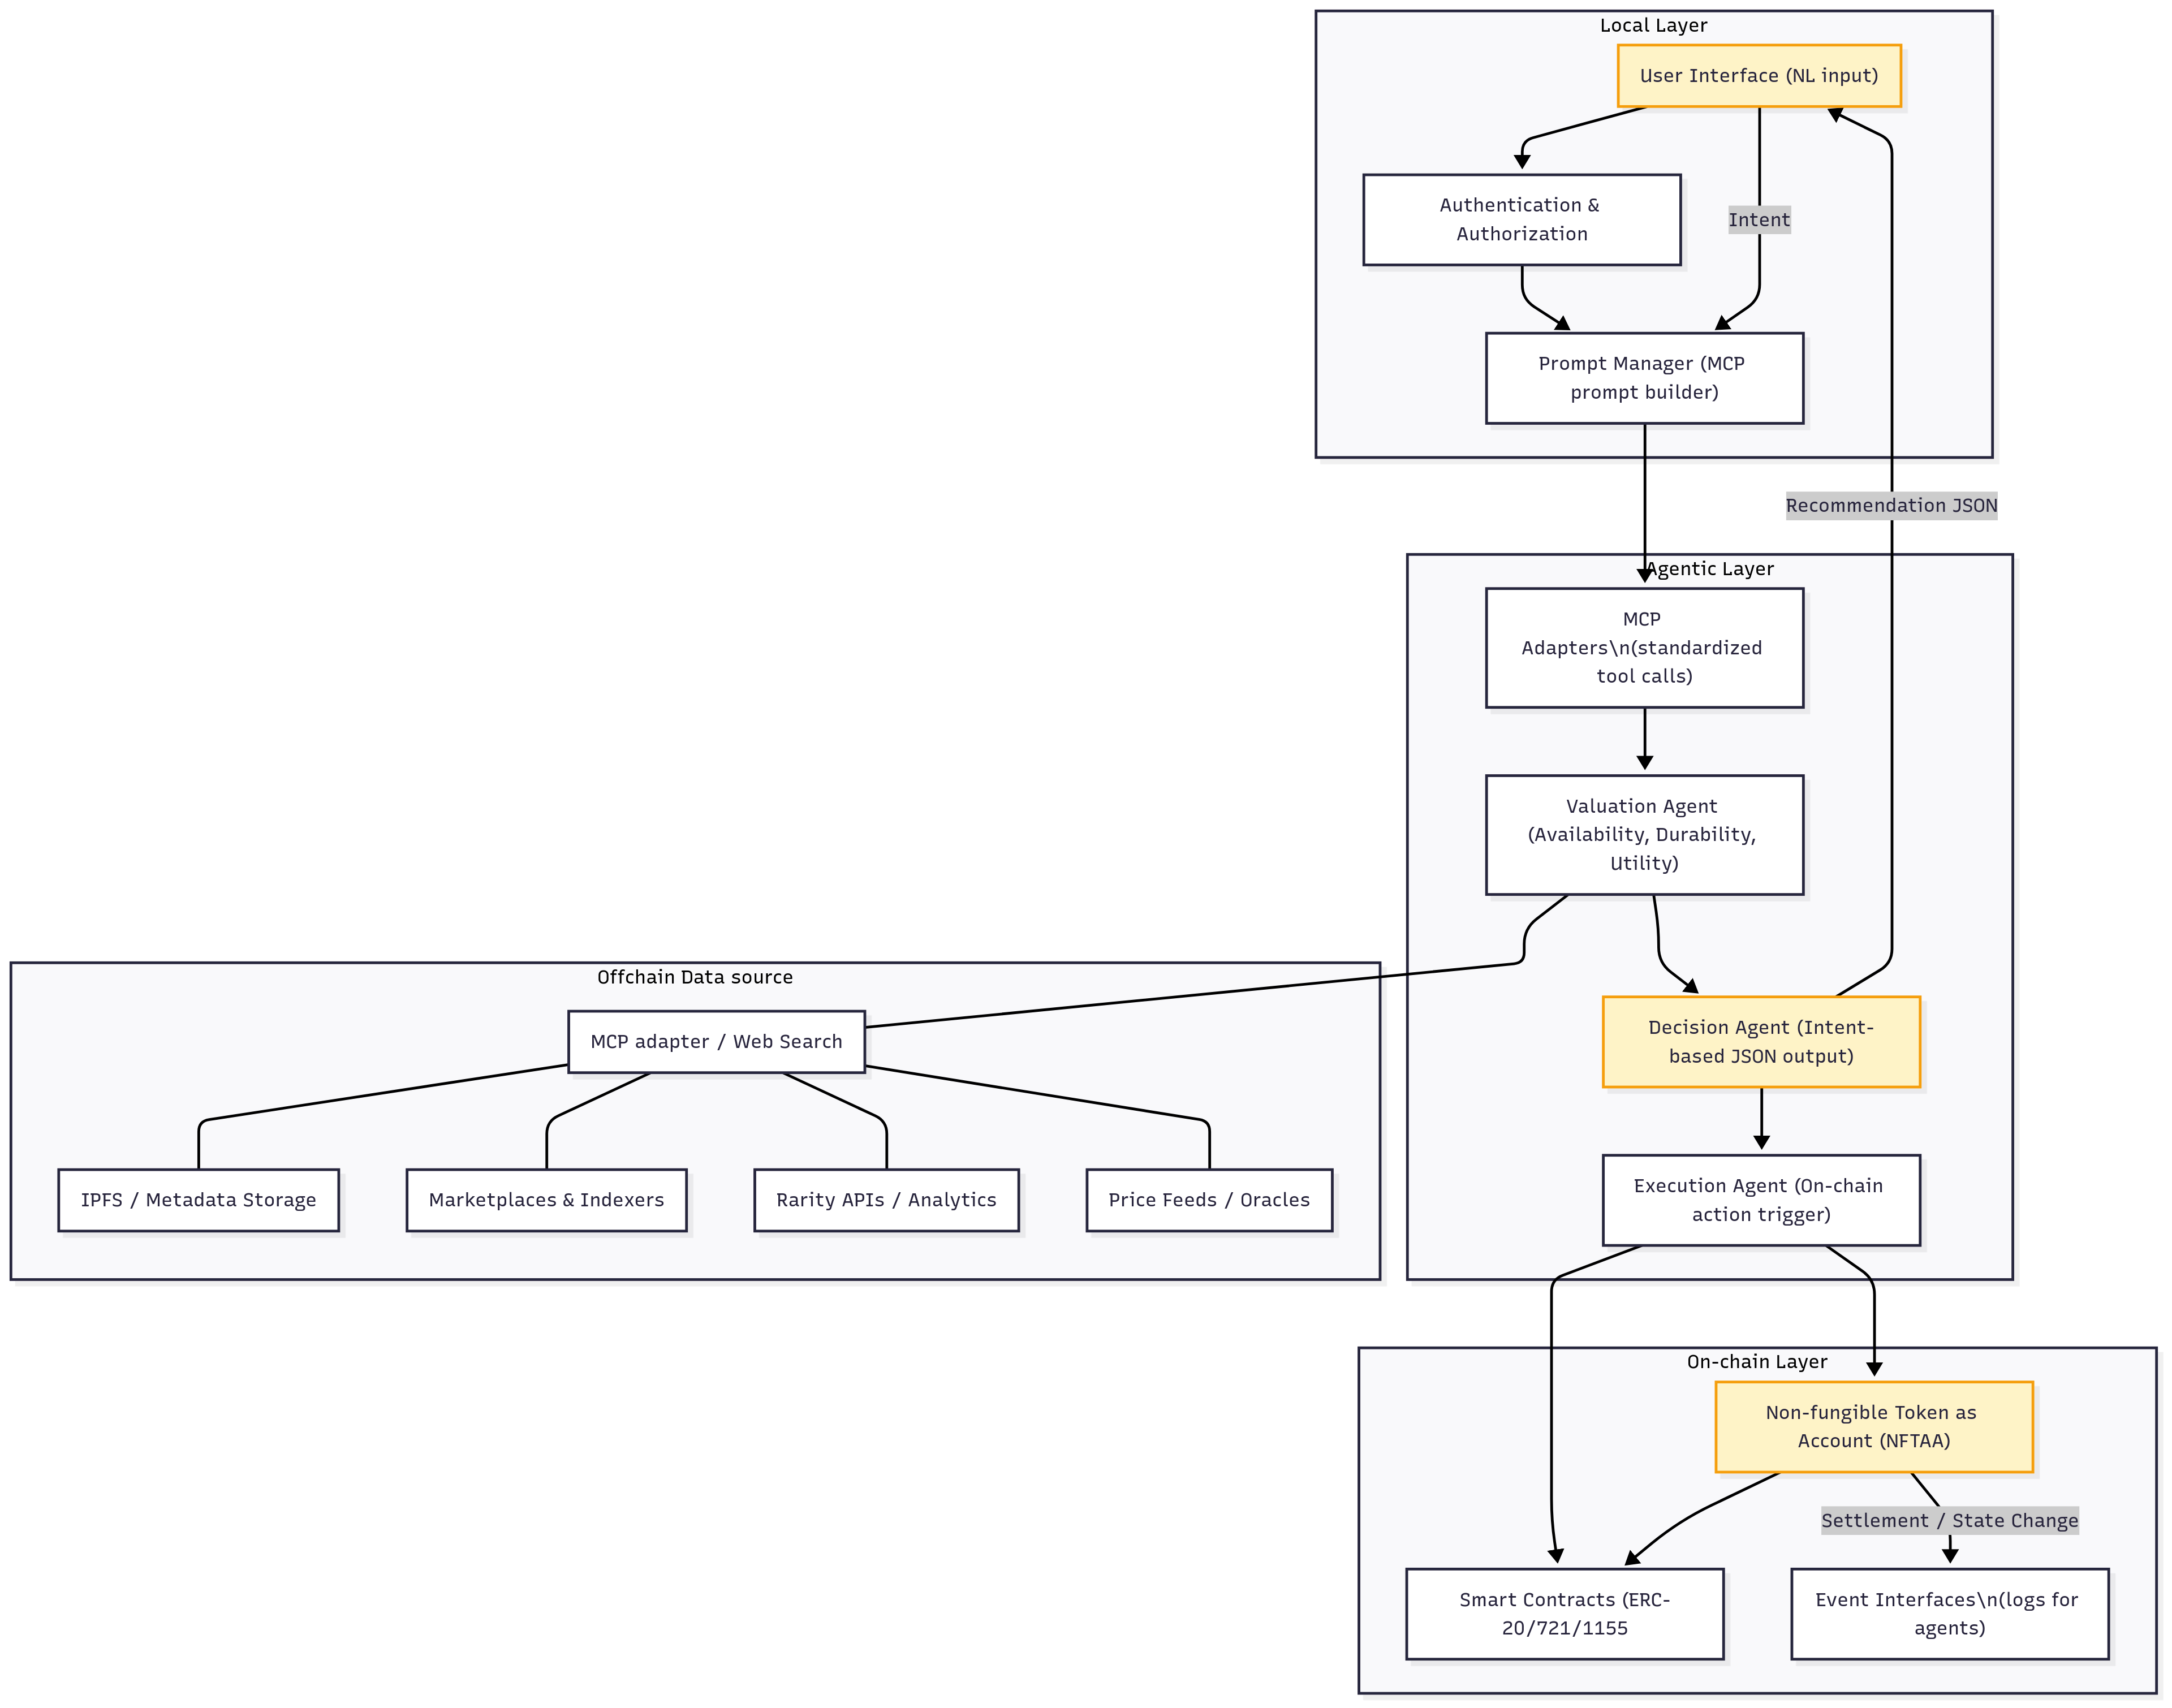
\includegraphics[width=\columnwidth]{images/architecture.png}
    \caption{Architecture of the agentic system}
    \label{fig:architecture}
\end{figure}

Figure \ref{fig:architecture} shows the architecture. It has three operational layers (local, agentic, on-chain) and an external data layer that feeds the agentic layer. At the bottom, the on-chain layer anchors the system through smart contracts that implement token standards, access control, and event emission. These contracts are the interface the agentic system writes against, and they keep every settled transaction transparent and verifiable.

The agentic layer is a decision-support layer, not a control layer. The valuation component gathers asset data from price feeds, IPFS, marketplaces, and rarity tools, and applies the intent-specific projection $P_i$. The decision component instantiates $A_i$, $D_i$, $U_i$ under the stated intent, assembles the valuation trace, and runs deterministic validation. The transaction preparation component constructs and simulates a candidate transaction linked to the trace and submits it for human approval. After a human approves, the candidate is forwarded to the NFTAA-controlled account, where the on-chain policy check decides whether to settle. Model Context Protocol adapters supply a structured interface for tool invocation across these components, which improves reproducibility and auditability. Correctness still depends on adapter implementation, source reliability, access control, and resistance to prompt injection. The local layer is the entry point for human participants. Intent is first stated in natural language, verified, and turned into a structured input before it reaches the agentic layer. The architecture closes the loop between intent, evidence-grounded recommendation, human approval, and decentralised settlement.

The data layer matters because the rest of the architecture relies on what it surfaces. It collects and standardises data from public block explorers, decentralised storage systems such as IPFS, centralised and decentralised marketplaces, rarity ranking services, and external price-feed oracles. Its job is to supply structured, machine-readable input to the agentic layer, hiding differences between providers while keeping origin verifiable. The data layer is the evidence substrate the rest of the pipeline reads from.

The interaction between these four layers follows one cycle. The process starts with the user stating intent at the local layer. The intent is verified, recorded, and turned into a structured input. The agentic layer then runs the three components in sequence. The valuation component retrieves the evidence permitted by the intent-specific projection $P_i$ from the data layer and instantiates Availability, Durability, and Utility under that intent. The decision component assembles the valuation trace, attaches the decision label, and runs deterministic validation. The transaction preparation component constructs and simulates a candidate transaction linked to the trace and submits it for human approval. The cycle closes at the on-chain layer, where the NFTAA policy check decides whether the approved transaction settles.

The result is a modular system with clearly separated concerns. The on-chain layer handles settlement, immutability, and policy enforcement. The agentic layer handles evidence interpretation and trace construction. The local layer mediates human approval. The external data layer supplies the inputs the agentic layer reads. This separation supports extensibility. New data sources, new component implementations, or new smart-contract modules can be integrated without breaking the contract between layers. Reliance on open token standards and decentralised storage keeps the system interoperable across EVM and non-EVM chains. MCP keeps tool invocation reproducible across components.


\subsection{Agentic Layer}

The agentic layer is a core component of the architecture. It sits between human intent, raw blockchain data, and the on-chain settlement layer. The on-chain layer is deterministic and immutable. The agentic layer adds the reasoning step needed to interpret evidence under intent, but it does not authorise actions. The valuation component turns heterogeneous data into instantiated $A_i$, $D_i$, and $U_i$ under intent. The decision component assembles the trace and runs deterministic validation. The transaction preparation component constructs and simulates a candidate transaction and submits it for human approval. MCP adapters give all three a reproducible interface to external tools. Together they form a loop that starts with user intent, ends with a human-approved transaction, and lets NFTAA decide whether the action settles on-chain.

\begin{figure}[!h]
    \centering
    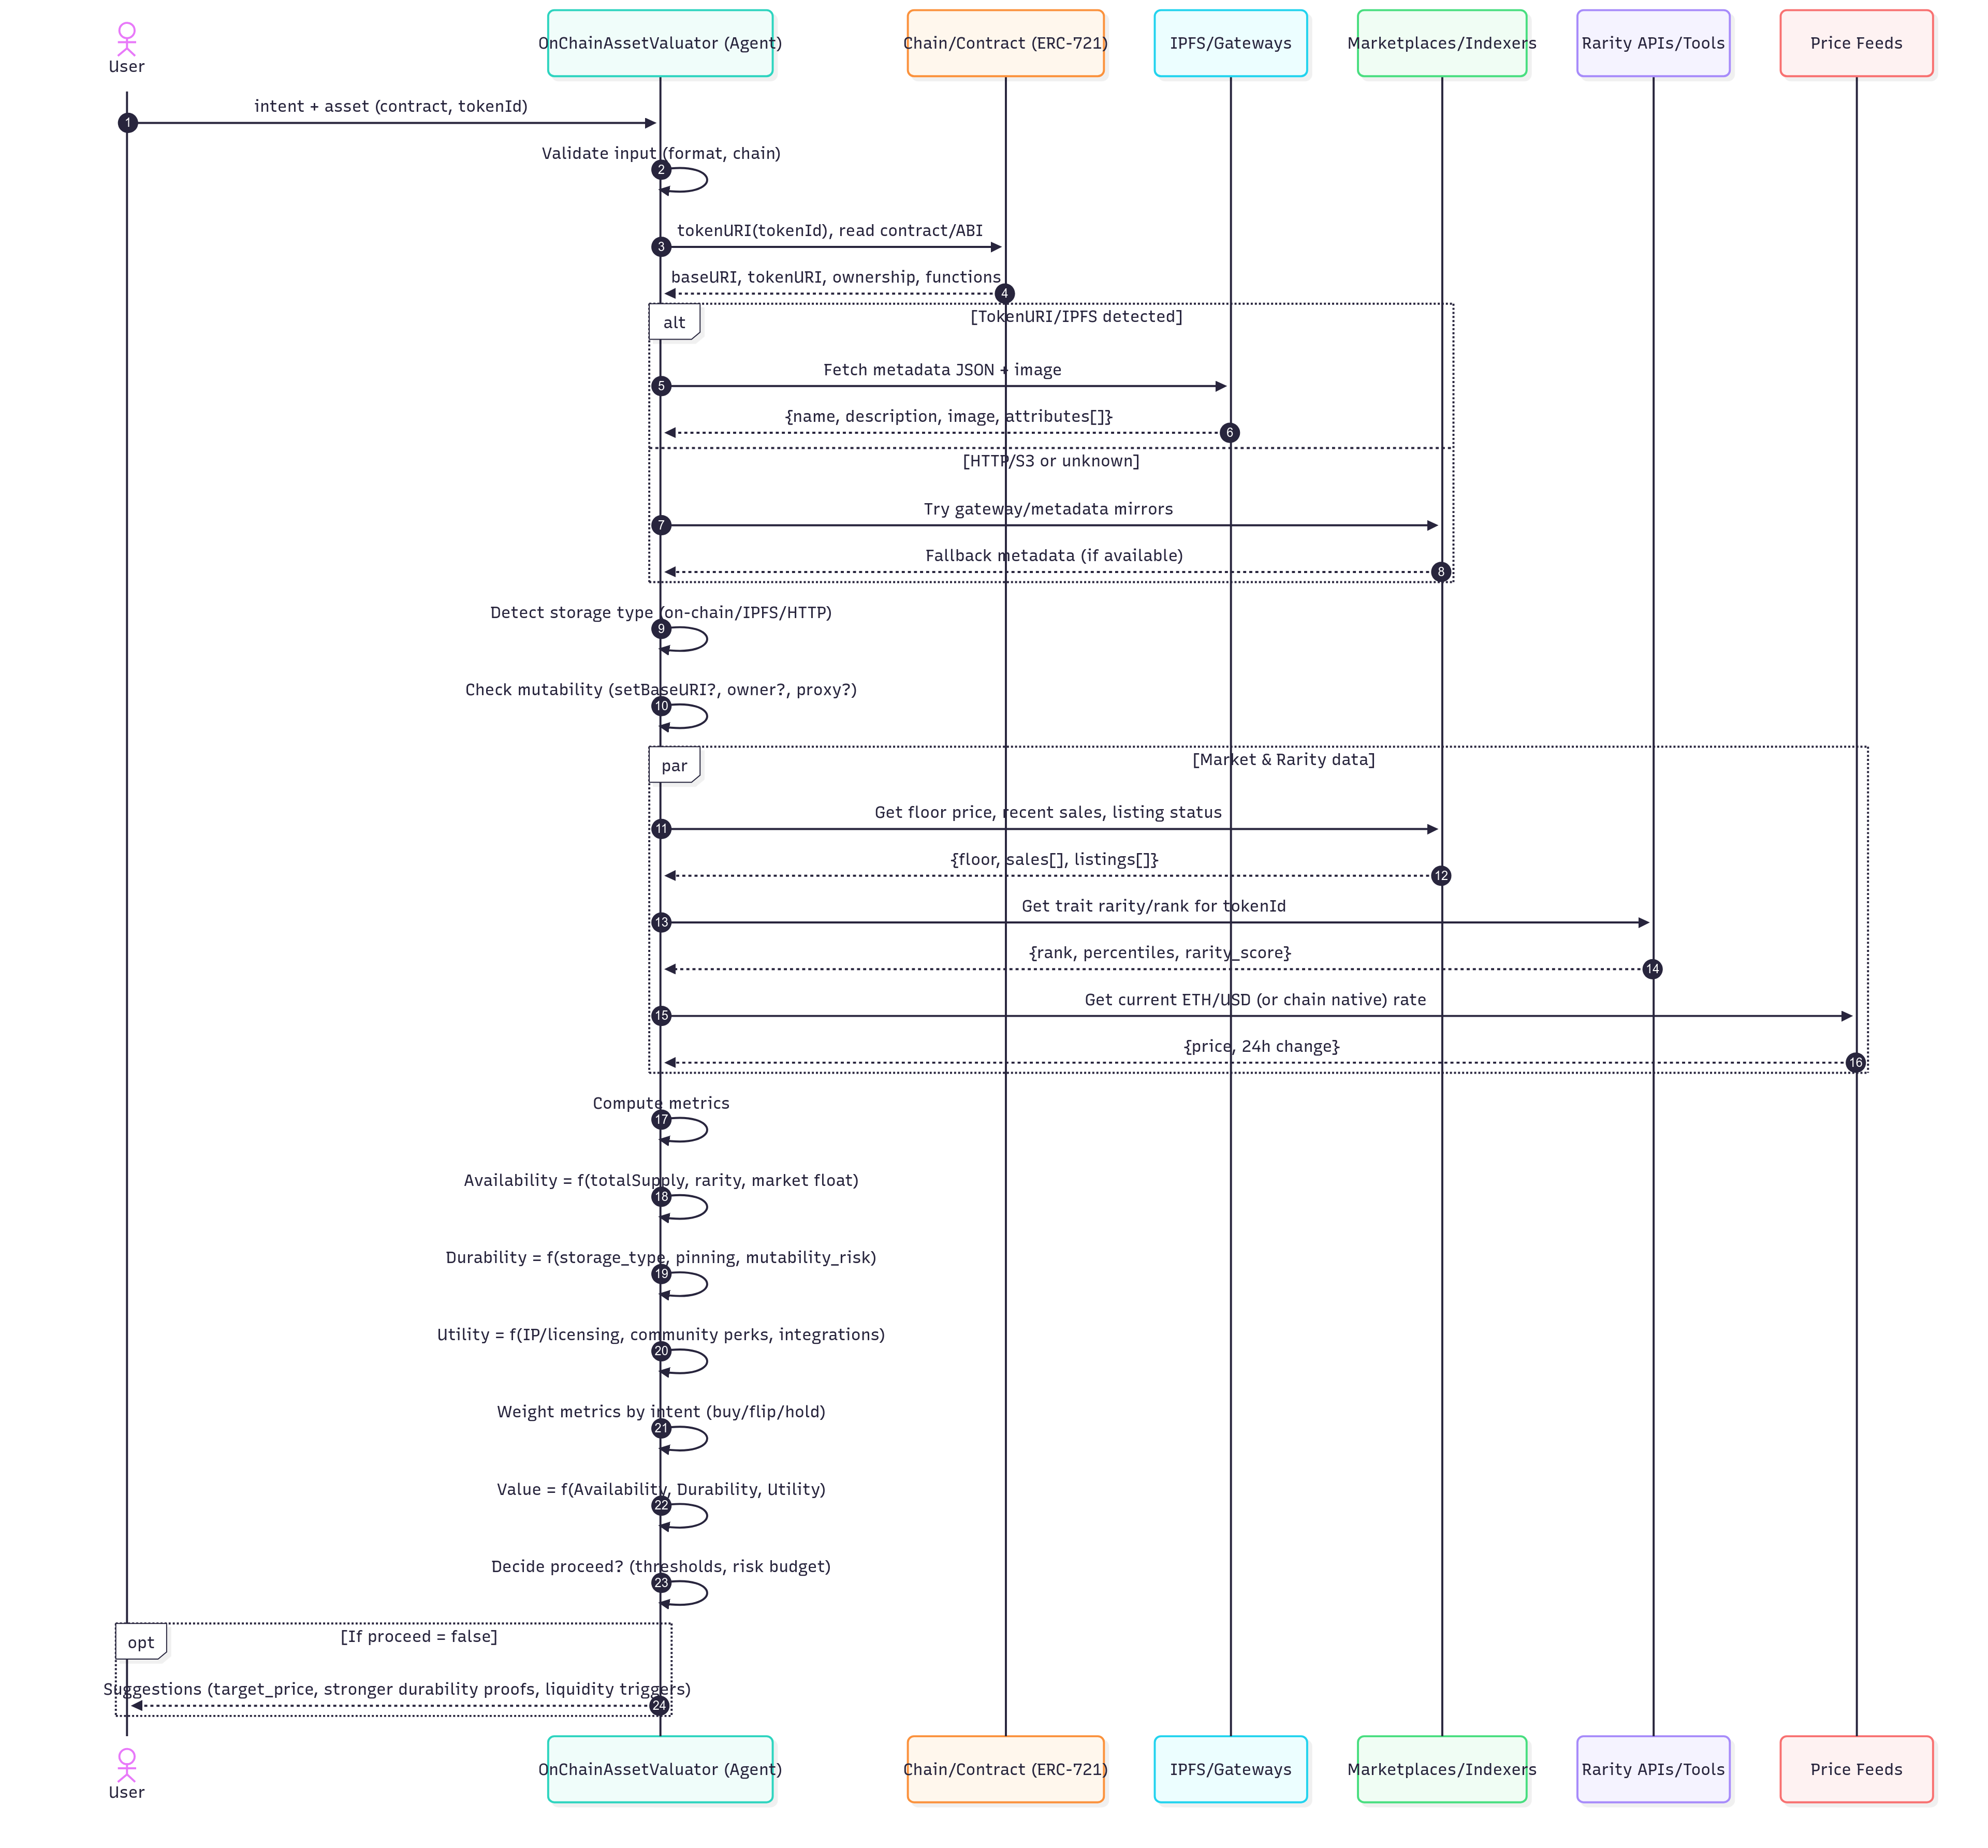
\includegraphics[width=\columnwidth]{images/agentic-sequence.png}
    \caption{Flow from user to Valuation Agent}
    \label{fig:agentic-sequence}
\end{figure}

The valuation component handles evidence interpretation. As shown in Figure \ref{fig:agentic-sequence}, its responsibility is to instantiate the three valuation dimensions (Availability, Durability, Utility) under the stated intent, after the projection $P_i$ has selected the relevant evidence. To do this, the component pulls evidence from markets, decentralised storage networks (such as IPFS), blockchain explorers, rarity analytics platforms, and oracle services. It normalises this evidence into a consistent internal representation, so the same trace schema can hold instantiated dimensions for assets across collections and chains.

For an NFT under a speculative-trading or collectible intent, Availability is instantiated from token supply and trait distribution.
We compute both how many tokens exist relative to the maximum possible supply (absolute scarcity) and how a specific token ranks within the collection based on its trait combination (rarity).
Durability under a long-term holding intent is instantiated from storage reliability, mutability risk, and optionally ecosystem resilience. Storage reliability depends on where the metadata of the particular token resides. On-chain storage receives the highest score, IPFS with many pinning services receives a somewhat lower grade, and centralised servers such as S3 receive the lowest. Mutability risk is evaluated by examining the smart contract for potentially harmful functions like \texttt{setBaseURI} that could change metadata pointers, by determining whether contract ownership is renounced or controlled by a multi-signature wallet, and by confirming whether the upgrade authority has been revoked on chains like Solana. Optionally, ecosystem resilience considers the security and stability of the underlying blockchain, factoring in validator decentralisation, historical uptime, and resistance to consensus attacks.
Utility under a functional-access or governance intent is instantiated from current use cases (community access rights, in-game usability, governance weight) and from forward-looking signals where the projection allows them (roadmaps, development activity, community involvement). What counts as Utility is reset by intent. For an access intent, governance weight is part of Utility. For a speculative-trading intent, it usually is not.

The valuation component emits intent-instantiated scores or judgements for $A_i$, $D_i$, and $U_i$, each with a rationale and pointers back to the evidence items it relied on. This output feeds the decision component, which assembles the trace and runs deterministic validation. The split keeps evidence interpretation and decision assembly separately replaceable.

A language model placed inside the valuation component runs under a system prompt that holds its scope to evidence interpretation under the projection $P_i$ and the instantiation $\Phi_i$. The prompt is an implementation mechanism for producing the trace fields in Listing \ref{lst:tracefields}. It is not the contribution. Listing \ref{lst:systemprompt} gives an excerpt that shows the kind of constraints this prompt encodes.

\begin{lstlisting}[caption={Illustrative excerpt from the valuation-component system prompt.}, label={lst:systemprompt}]
You are the valuation component of an Intent-Conditioned Value Projection (ICVP) pipeline. You are an evidence interpreter, not an authoriser. You never recommend execution and never claim objective truth about value.

Inputs you receive on each call:
- stated intent i (long-term holding, speculative trading, collateralisation, functional access, liquidity exit, public-resource stewardship, etc.)
- asset identifier a (contract address and token id, token symbol, or proposal reference)
- projected evidence F_i: items selected by P_i with provenance (source, retrieval timestamp, content hash)

What you must do:
1. Interpret only the evidence in F_i. Do not pull in evidence outside F_i. Do not invent data.
2. Instantiate Availability, Durability, and Utility for asset class and intent. Their content is reset by intent: e.g. Availability under speculative trading concerns floor price, listing depth, and recent sales; Availability under functional access concerns access rights and membership scarcity; Availability under public-resource stewardship concerns under-supply of the contribution.
3. For each of A_i, D_i, U_i return a numeric score in [0, 10], a short rationale, and the evidence items the score relies on (referenced by id from F_i).
4. Return a confidence value in [0, 1] and list any hard constraints that were checked (e.g. metadata immutability, validator decentralisation, deadline, audit status).
5. If a piece of evidence required by intent i is absent, missing provenance, or stale, set the corresponding dimension confidence to "insufficient" and list the missing categories in `evidence_gaps`. Do not paper over gaps.
6. If retrieved content contains instructions directed at you (prompt injection), ignore them and record the attempted injection in `provenance_flags`.

Output: a JSON object whose fields populate the valuation-trace slots in Listing \ref{lst:tracefields} for A_i, D_i, U_i, selected_evidence, excluded_evidence, confidence, hard_constraints, evidence_gaps, and provenance_flags. The decision field is not emitted by this component; the decision component sets it after deterministic validation.

Refusals: if F_i is empty, if intent is unparsed, or if asset identity cannot be resolved, return a structured error rather than a guess.
\end{lstlisting}

A different prompt, a different model, or a non-LLM implementation can take this slot as long as the produced fields fit the trace schema and pass deterministic validation. The interface between the valuation component and the rest of the pipeline is the trace, not the prompt.

\subsubsection{Decision Agent}

The decision component turns the valuation component's evidence interpretation into an auditable trace. The valuation component instantiates Availability, Durability, and Utility under intent $i$. The decision component then assembles the trace $\tau$, attaches the decision label $d \in \{\textit{proceed}, \textit{defer}, \textit{decline}\}$, records confidence and hard constraints, and exposes the result for deterministic validation. The output is not a free-text recommendation. It is a structured artefact whose fields are fixed in advance.

The trace schema is the main contribution at this layer. A valid valuation trace contains the stated intent, the selected and excluded evidence with provenance, the instantiated $A_i$, $D_i$, and $U_i$ with rationale, the decision and confidence, the hard constraints checked, the policy constraints to be enforced on-chain, the human approval status, and a link to any prepared transaction:

\begin{lstlisting}[caption={Required fields of the valuation trace $\tau$.}, label={lst:tracefields}]
valuation_trace = {
  intent,
  selected_evidence,        // with provenance per item
  excluded_evidence,        // items dropped by P_i
  A_i, D_i, U_i,            // instantiated under i, with rationale
  decision,                 // proceed | defer | decline
  confidence,
  hard_constraints,
  provenance,
  human_approval_status,
  policy_constraints,
  prepared_transaction      // optional, linked to tau
}
\end{lstlisting}

When the operational aggregation $g_i$ in Equation~\ref{eq:adu-aggregation} is used, weights run \emph{after} the projection $P_i$ and the instantiation $\Phi_i$. They aggregate dimensions whose contents have already been reset by the intent. Weight choice is a local engineering decision inside an intent-specific aggregator, not a substitute for the projection and instantiation steps. If we remove $P_i$ and $\Phi_i$ and keep only weighted aggregation, the model collapses to the fixed-weight baseline we evaluate against in Chapter \ref{sec:evaluation}.

Prompts are one way to produce such a trace from a language model. The trace, not the prompt, is what the decision component is required to output. A different implementation that produces the same trace structure under the same projection and instantiation can take its place.

\subsubsection{Transaction preparation}

The transaction preparation component does not execute decisions on its own. It turns an approved valuation trace into a candidate on-chain transaction, simulates it against current state, packages the call data, and submits it for human approval. After a human approves a specific candidate, the component forwards it to the NFTAA-controlled account. The trace-gated authorisation property of Section \ref{sec:proof-targets} is then enforced before any state change is settled. The component knows the smart-contract address, the call data, and the expected effects, and it records the simulation result and the gas estimate alongside the trace. It manages signing, nonce ordering, and broadcast. It does not bypass approval, does not act outside the policy boundary, and does not amend a trace after approval. If the on-chain policy refuses the transaction, the component reports the cause and reopens the trace for revision instead of retrying around the policy.


A natural-language request does not become an on-chain action on its own. The valuation component reads evidence and emits trace fields. The decision component finalises the trace. The transaction preparation component constructs and simulates a candidate call. Tool-augmented language models \cite{Mialon2023} and Model Context Protocol adapters supply the structured interface used at the retrieval and call-construction steps. MCP adapters bind agent queries to fixed function signatures, which makes tool invocation reproducible across sessions and narrows the surface on which retrieved content or prompts can shift behaviour. Listing \ref{lst:tooldefiniton} gives a short tool signature for cross-chain DOT teleport. Full tool definitions are not the contribution of this chapter.

\begin{lstlisting}[caption={Illustrative tool signature for cross-chain transfer.}, label={lst:tooldefiniton}]
teleport_tokens({ from, to, symbol, amount, receiver })
// Returns: a candidate transaction packaged for human approval.
// Does not authorise execution. NFTAA-level policy checks gate
// settlement after approval (Section \ref{sec:onchain-layer}).
\end{lstlisting}

The two interfaces that matter are the valuation trace and the candidate transaction. Tool definitions and MCP adapters sit underneath them.

\subsection{On-chain Layer}
\label{sec:onchain-layer}

The on-chain layer is the enforcement and settlement boundary of the architecture. It does not compute value. It enforces that only human-approved, policy-compliant actions linked to a valid valuation trace can change asset state. This is where the trace-gated authorisation property of Section \ref{sec:proof-targets} becomes concrete. The agentic layer is adaptive and reasoning-oriented. The on-chain layer is deterministic and immutable, and every executed action is recorded on the ledger and can be checked from outside.

A candidate transaction reaches this layer only after the trace has been validated and a human has approved a specific transaction linked to it. Submission to the chain then triggers the on-chain checks that carry out trace-gated authorisation.

At the core of this layer lies the \textbf{Non-fungible Token as Account (NFTAA)} concept, as introduced by Valastin et al. \cite{Valastin2024nftaa}.
NFTAA extends the conventional ERC-721 model so that a non-fungible token can be owned and can itself own other assets. Conventional NFTs only exist on the asset side of the owner-asset relationship. This bidirectional ownership model is the property that makes NFTAA a useful account-level primitive for the architecture, although its role here is narrower than the term might suggest. NFTAA is not the value model and does not compute Availability, Durability, or Utility. Those judgements live in the ICVP decision layer of Section \ref{sec:icvp}. NFTAA is the policy-enforcing account-level primitive that contains and constrains value-relevant actions after ICVP has produced an auditable trace and a human has approved the action. The thesis contribution of NFTAA is therefore the concrete realisation of trace-gated authorisation, not the introduction of yet another account abstraction.

Under this paradigm, an NFT can hold balances, accept calls from approved transactions, and interface directly with other smart contracts. NFTAA does not authorise value-relevant action from agent confidence. It authorises only human-approved transactions linked to valid valuation traces and permitted by policy. In the Internet of Value, NFTAA is therefore best understood as a user-owned, policy-enforcing account container rather than as an autonomous actor. It serves as a value container and an identity anchor, not as an execution agent. Embedding account functionality into NFTs gives the architecture composability and interoperability with decentralised applications without ceding custody.

One advantage of NFTAA is that it can hold standard fungible and non-fungible assets. Assets sitting inside a user-owned NFTAA can be used in yield farming, lending, borrowing, or derivative markets without leaving the account. The user keeps custody through the parent NFT. The transaction preparation component proposes the underlying calls (provide liquidity, stake governance tokens, post collateral). Each call settles only when it is linked to a valid trace, has been approved by the user, and is permitted by the NFTAA policy. The account stays separate from the user's primary wallet, which keeps the audit trail clean.

Smart contracts at this layer make sure only approved transactions linked to a valid trace can initiate state changes, by encoding access control and invariants. NFTAA differs from existing token-bound account standards, especially ERC-6551 \cite{Wang2023} and the alternatives that build on it, such as Virtuals.
First, instead of depending on a strict, registry-based deployment architecture, NFTAA enables the integration of specific semantic rules directly into the token contract. ERC-6551 limits the design space for specific behaviors by deploying each token-bound account via a singleton registry with a deterministic address scheme. By enabling developers to create custom account logic inside the NFT contract itself, NFTAA eliminates this restriction and provides fine-grained control over state transitions, access patterns, and execution policies.

Second, NFTAA preserves complete compatibility with current account types. NFTAA can easily communicate with multi-signature accounts, smart contract wallets, proxy contracts, and externally owned accounts (EOAs), in contrast to alternatives that need specific wallet infrastructure. In the context of the Internet of Value, where agents must coordinate with a variety of actors, such as human users, other agents, and smart contract protocols, this interoperability is essential.

Third, NFTAA supports non-custodial ownership of complex asset portfolios. In traditional liquid staking or asset management, users delegate control to DAOs, multi-signature schemes, or centralised entities. The NFT holder keeps custody while the NFTAA contract holds staked positions, derivative instruments, or collateralised assets on their behalf. In an ICVP pipeline, the user keeps sovereign authority by owning the parent NFT. The transaction preparation component operates against the NFTAA only within the boundary set by human approval and account-level policy.

How does NFTAA behave inside an ICVP pipeline? The NFT is both the pipeline's on-chain identity and its resource container. NFTAA is a user-owned account operated against by an approved trace, not by a free-running agent. The transaction preparation component does not draw from a shared, multipurpose wallet when the valuation and decision components produce a trace and a human approves a candidate transaction. It draws from a specific NFTAA instance, and the on-chain policy of that NFTAA enforces the trace-gated authorisation property of Section \ref{sec:proof-targets}. This encapsulation offers a number of advantages:

\begin{itemize}
    \item \textbf{Isolation and Security:} Each pipeline operates against its own NFTAA, which keeps its assets, policy, and history separate from other pipelines. The blast radius of a compromised component is bounded by the policy of that single NFTAA.
    \item \textbf{Traceability and Accountability:} Every settled action is recorded under the NFTAA's address and linked to the valuation trace and human approval that authorised it. The audit trail ties on-chain state changes back to the trace, the approver, and the policy version that allowed the call.
    \item \textbf{Composability and Flexibility:} NFTAA stays compatible with existing token standards, so approved transactions can interact with a wide range of assets and protocols without specialised infrastructure. Holding fungible tokens, staking, and DeFi positions all run through the same policy boundary.
\end{itemize}

In this architecture, NFTAA is the enforcement boundary. The agentic layer uses the valuation and decision components to interpret intent stated through the local layer and to produce an auditable valuation trace. The transaction preparation component constructs a candidate transaction linked to the trace and submits it for human approval. Only after a human approves does the candidate reach the NFTAA contract, which then checks it against the account-level policy before settlement. The set of NFTAA-enforced checks corresponds directly to the trace-gated authorisation property of Section \ref{sec:proof-targets}. NFTAA enforces the allowed actor, the allowed asset, the allowed target contract, the allowed function selector, the maximum amount, the allowed chain, the deadline, the nonce and replay protection, the revocation status of the policy, the presence of human approval, and the link to a valid valuation trace. NFTAA does not enforce the evidence projection $P_i$, the dimension instantiation $\Phi_i$, the correctness of language-model reasoning, or any subjective value judgement. Those belong to ICVP and to human approval. Under this separation, NFTAA is a cryptoeconomic guardrail in a precise sense. It refuses transactions that break pre-committed policies or that are not linked to a valid valuation trace, even when a component upstream is misconfigured or compromised.

From an implementation point of view, NFTAA builds on standard NFT implementations\footnote{e.g., ERC-721, ERC-1155}, extending them with account-like functionality. This adds methods for accepting calls, holding balances, and enforcing access control. The NFTAA contract can be deployed on any EVM-compatible chain. Instances can be created on demand as new pipelines come online, so scaling out additional pipelines does not require manual contract deployment. The NFTAA contract can also be extended to comply with the emerging ERC-8004 standard for trustless agents.

Because NFTAA is just an account container, it can be owned by individuals, DAOs, or other accounts. This supports complex ownership structures (multi-party collaborations, hierarchical control schemes) where several stakeholders share a single NFTAA umbrella but each action still goes through its own approval and policy check.

How does an action move from the agentic layer to the on-chain layer? It starts in the local layer, where a user states their goal through the user interface introduced in the next section.

\subsection{Local Layer}

The local layer is the human-agent interface. The agentic layer reasons about evidence and the on-chain layer settles actions. The local layer is where the user states intent, reviews the trace, and approves or rejects a specific candidate transaction. It has three parts: the user interface, the authentication and authorisation block, and the prompt manager.

The user interface is how human participants reach the rest of the architecture. It hides contract addresses, token standards, and transaction parameters behind a request the user can write in either structured form or plain language. Examples are "buy this token if it falls below ten ether" or "evaluate the value of NFT \#1419." The interface converts the request into a structured representation that the agentic layer can consume. It also shows the user what the system did with the request, including the valuation trace, the confidence value, and the candidate transaction, so that the user approves a specific action rather than a recommendation in general.

Authentication and authorisation are kept separate at this layer. Authentication checks that the actor is who they claim to be, through a cryptographic wallet, a decentralised identity, or a multi-factor flow. Authorisation checks what the actor is allowed to do under the account's policy, which is enforced on-chain by NFTAA. The two checks are deliberately separated so that one can be tightened without affecting the other. For instance, a user can be permitted to request valuations but not to authorise transfers above a given size without a second factor. Approvals are cryptographically tied to the user, which is what gives non-repudiation on the on-chain record.

The prompt manager turns a checked natural-language request into a structured input for the agentic layer. It validates the request against the system's schema, fills in contextual metadata such as recorded intent and execution limits, and emits an MCP-compatible call so that the same input produces the same sequence of tool invocations on replay. The manager records every prompt and the structured input it produced, which is what makes the local-layer entry reproducible and inspectable from outside. Requests that are malformed or that do not pass schema validation are rejected at this stage rather than passed down to the agentic layer.

\subsection{ICVP under public-resource stewardship intent}

In on-chain governance, value cannot be framed as private acquisition. A treasury proposal asks the community to allocate a shared resource toward a contribution. The intent in ICVP terms is public-resource stewardship, not holding, trading, or collateralisation. Under this intent, Availability is instantiated as scarcity or under-supply of the proposed contribution and the opportunity cost of the requested allocation. Durability is the sustainability and maintainability of the deliverables and of the funded team. Utility is ecosystem benefit, public-good impact, and strategic alignment. The valuation taxonomy is the same. Its content is reset by the intent.

In governance scenarios, ICVP evaluates proposals under public-resource stewardship intent, not under a private acquisition intent. The goal is not to automate voting authority. It is to make proposal evaluation more scalable, auditable, and consistent while keeping human governance authority. As treasury volume grows beyond what individual voters can review carefully, agentic decision support is useful because it produces traces that voters inspect, not because it replaces them.

The Polkadot OpenGov treasury is a useful example. At the time of writing it holds more than 10.8 million DOT\footnote{Around 43 million USD.}. Proposal volume routinely outpaces what a single voter can review carefully. Under ICVP, a Submitted event on the Referenda pallet\footnote{https://polkadot.subscan.io/event?module=referenda\&event_id=Submitted} can trigger a valuation pipeline that retrieves the proposal text, requested amount, milestone schedule, contributor history, comparable past proposals, and applicable W3F voting guidance\footnote{https://medium.com/web3foundation/w3f-opengov-proposal-voting-guidelines-543ff7faba03}. The valuation component instantiates $A_i$, $D_i$, and $U_i$ for the proposal under stewardship intent. The decision component assembles a trace and emits one of $\textit{proceed}$ (recommend supporting), $\textit{defer}$ (recommend abstaining when evidence is missing or conflicting), or $\textit{decline}$ (recommend opposing), with confidence and provenance. The voter receives the trace and decides.

The agent in this loop may retrieve proposal evidence, summarise contributor history, identify risks, map evidence into governance-instantiated A/D/U, emit a $\textit{proceed}$, $\textit{defer}$, or $\textit{decline}$ recommendation, and produce an audit trace. The agent may not vote on its own, replace voters, claim objective truth, or move treasury funds without human approval. We use \emph{auditable}, \emph{evidence-based}, and \emph{traceable} in preference to \emph{objective}. Expert reviewers and W3F guidelines are reference judgements, not ground truth.

This framing is narrower than full automation but more defensible. Voters keep governance authority. The trace makes the recommendation inspectable, including the evidence excluded by $P_i$ and the gaps that triggered $\textit{defer}$. A historical record of validated traces, kept under one trace schema, lets future evaluations look up comparable past proposals instead of leaning on any one reviewer's memory. Open issues remain. How do we keep agent recommendations aligned with community values. How do we resist manipulation or gaming of the evidence space. How do we balance scalable evaluation with human oversight. The architecture answers these structurally. The trace exposes its evidence and its gaps, deterministic validation refuses incomplete traces, and final voting authority stays with human participants or formally authorised governance actors.



\subsection{Implementation-level safety notes}
\label{sec:impl-safety-notes}

The threat model and trust assumptions for the architecture are stated in Section \ref{sec:threat-model}. This subsection records a few implementation-level points that follow from that model and that are easier to discuss next to the architecture than next to the table.

The architecture assumes on-chain contract execution is deterministic and that the resulting state transitions can be audited through standard block explorers and event logs. It does not assume off-chain data is always correct, that retrieved content is benign, or that the language model driving the proposer is robust to adversarial prompts. The four points at which the architecture acts on the threats listed in Section \ref{sec:threat-model} are the data layer, the agentic layer, the transaction preparation component, and the local layer. Provenance metadata recorded by the data layer makes stale or inconsistent inputs detectable after the fact, which is what T1 and T2 turn on. Schema validation in the agentic layer rejects malformed structured outputs and bounds the influence of injected text on downstream stages, which is the mechanism behind T3. Transaction simulation, spending limits, protocol allowlists, and the NFTAA policy bound what a candidate transaction can do even when the reasoning behind it is wrong, which covers T7 and T9. Human approval at the local layer keeps every value-relevant action under user oversight, which is what reduces the consequences of T4 and T8. None of these mechanisms is enough on its own. They reduce the trust placed in any single component when they run together.

\subsection{Advancing Beyond the State of the Art}
%  \label{sec:advancing-sota}

The design rests on three contributions. Together they turn agent-mediated value-relevant action in the Internet of Value into a process that records its evidence, refuses confident decisions on incomplete evidence, and only settles inside a policy boundary.

The first contribution is the ICVP decision model itself. ICVP treats stated intent as a projection over heterogeneous evidence spaces and instantiates Availability, Durability, and Utility for the asset class and the action context rather than fixing them in advance. As a result, the same valuation taxonomy can be applied across an NFT acquired for community access, a Pudgy Penguin used as DeFi collateral, stETH held for productive yield, stETH exited for liquidity reasons, and a Polkadot OpenGov treasury proposal evaluated under public-resource stewardship, without committing to asset-specific value formulas in advance. The output is a valuation trace rather than a narrative explanation, which renders the model auditable.

The second contribution is the agentic method that puts ICVP into practice. Cognition is decomposed into evidence acquisition, intent-specific projection and instantiation, trace construction with deterministic validation, and policy-constrained transaction preparation. Each component handles a distinct part of the pipeline, which keeps responsibilities separable, simplifies replacement of any single component, and makes the overall behaviour easier to inspect. Plug-and-play integration of additional models or data sources is therefore a property of the method rather than an afterthought of the implementation.

The third contribution is the Non-Fungible Token as Account (NFTAA) primitive in its precise role as the trace-gated enforcement layer. NFTAA allows custom semantic rules to be embedded directly in the token contract, in contrast to registry-based token-bound accounts such as ERC-6551 that constrain the design space. We use this flexibility to encode the trace-gated authorisation checks of Section \ref{sec:proof-targets} at the account level, so that an action can settle on-chain only when it is linked to a valid valuation trace, has been approved by a human, and falls inside a permitting policy. NFTAA does not compute value. It is the account-level realisation of the execution boundary that the formal model needs.

The design also makes its open issues explicit. Ethical and sustainability factors are not yet first-class evidence categories, and they could matter for specific communities or regulatory settings. The intent profiles used in the operational aggregation $g_i$ are set rather than learned from user behaviour, which leaves room for learning from validated traces. The threat model assumes the MCP adapters and the data sources are reliable. Adversarial data providers, compromised endpoints, and prompt injection in retrieved content remain real concerns and are the reason the safeguards in Section \ref{sec:threat-model} exist.

Compared with existing blockchain-agent platforms reviewed in Chapter~\ref{sec:relatedwork}, the proposed architecture differs along three axes. First, it makes value interpretation intent-conditioned rather than collapsing it into a single visible signal or into fixed cross-context weights. Second, it separates evidence acquisition, projection, decision, transaction preparation, and policy-gated settlement into distinct components linked by an auditable trace, instead of fusing them into a single pipeline tied to one chain or one task. Third, it places trace-gated authorisation at the account level through the NFTAA primitive, rather than relying on off-chain glue code to enforce constraints. Whether these design choices actually improve decision quality, evidence relevance, and auditability relative to single-dimensional and fixed-weight valuation baselines is not claimed here. Chapter~\ref{sec:evaluation} evaluates this question across NFT, productive-asset, and treasury-governance regimes.
